\section{Changes to the Task 1 Metamodels and Task 2 Transformations}
\label{sec:appendix}

This appendix lists changes to the Task~1 metamodels and Task~2 transformations
in the Task~3 pipeline, organised by artefact. The baseline is the Task~2
submission's metamodel appendix and design section. These describe three
QVT-Operational transformations (lowering, resolution and the estate pass
over the Resolved Deployments) and the Task~1-to-Task~2 metamodel changes.
Each subsection contains tables with one row per change, identifying the
affected classes and features and briefly explaining the reason.

The model was refined as it was applied to production: deploying the real
estate surfaced cases the model had to express, and the changes below came from
those cases. The tables group them by theme; changes that concern only the
model-driven implementation, not the model, form a group of their own. The
change set was derived from the repository's git history rather than a
comparison of complete models, so each row summarises a commit's effect.

File sizes indicate the extent of the changes. As submitted, the Project Intent
metamodel, which also holds the Platform Intent classes, has 137 classes and
441 features, the Resolved Deployment metamodel 133 classes and 619 features,
and the Pinned Inputs metamodel 15 classes and 67 features. The resolution
transformation has 4276 lines, 10 mappings and 305 queries, and the lowering
has 473 lines and 54 mappings, compared with about 1700 and 340 lines in the
Task~2 design section. The 134-line estate pass was removed. The Acceleo
module has 3772 lines.

\subsection{Source Metamodel (Project Intent)}
\label{sec:appendix-source}

The source metamodel defines what an author writes in a Project's files.
Figure~\ref{fig:mm-source} shows its Project Intent part. Changes fall into five
themes: how a \texttt{Process} reaches platform services, how it receives secrets,
the identity and placement constraints checked by the model, further forms of
\texttt{Process}, and the exposure, sign-in and observation of an
\texttt{Application}. The Platform Intent classes live in
the same \path{project-intent.ecore} file, and Section~\ref{sec:appendix-platform}
covers them separately.

\begin{figure}[!htbp]
\centering
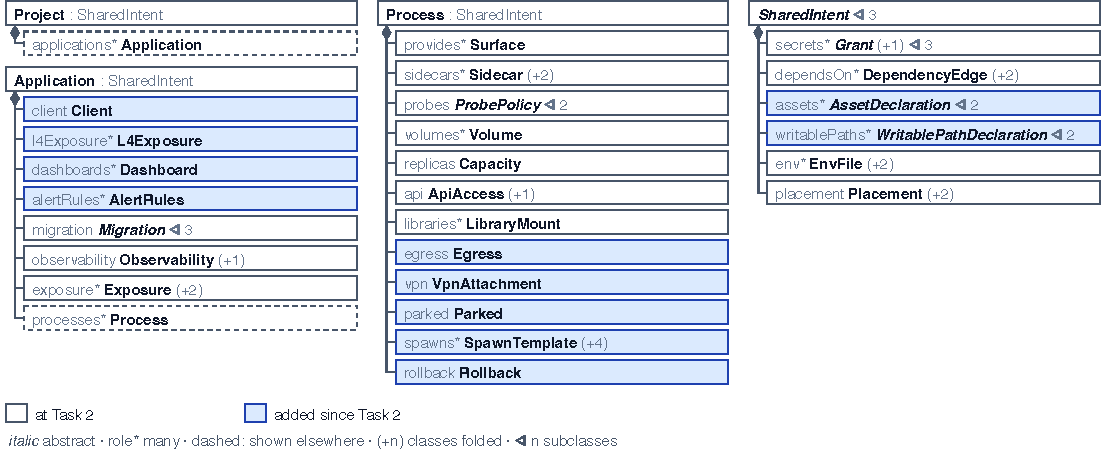
\includegraphics[width=\linewidth, keepaspectratio]{Figures/mm-source}
\caption{The Source Metamodel as Submitted}
\label{fig:mm-source}
\end{figure}

These changes keep authored documents small. Each new field records a choice
the author must make or a reason the model could not infer. No field is added
where a platform fact already determines its value.

\begin{table}[!htbp]
\centering
\footnotesize
\begin{tabular}{>{\raggedright\arraybackslash}p{\dimexpr0.22\linewidth-2\tabcolsep}>{\raggedright\arraybackslash}p{\dimexpr0.48\linewidth-2\tabcolsep}>{\raggedright\arraybackslash}p{\dimexpr0.30\linewidth-2\tabcolsep}}
\hline
\textbf{Change} & \textbf{What changed} & \textbf{Why} \\
\hline
\multicolumn{3}{l}{\textit{Reaching the platform's services}} \\
Process VPN attachment & \texttt{Process} gains \texttt{vpn}, a \texttt{VpnAttachment} holding one \texttt{forwardedPort}. Its image, credential and resource quantities come from Platform Intent. & The author specifies only the forwarded port, without tunnel details. \\
Internet egress & \texttt{Process} gains \texttt{egress}, containing \texttt{to} entries of \texttt{EgressTarget} and a required \texttt{reason}. & Default deny remains the rule; each exception has a declared reason for review. \\
Library mount & \texttt{Process} gains \texttt{libraries}: \texttt{LibraryMount} (\texttt{library}, \texttt{mountAt}, \texttt{subPath}) with a \texttt{LibraryAccess}. & A library is a directory on one node. The mount names it and requests access, which is checked against the grant. \\
GPU placement & Placement gains a structured \texttt{gpu} with a vendor and model. & One declaration selects and requests a card, so the request is derived without repetition. \\
\multicolumn{3}{l}{\textit{Secrets and keys}} \\
Declared secret keys & The flat key list becomes \texttt{KvKey}, a \texttt{name} with either \texttt{PlainKey} or \texttt{GeneratedKey}. \texttt{GeneratedKey} holds \texttt{generate}: \texttt{bytes} and an \texttt{encoding} of \texttt{KeyEncoding}. & A platform-generated key is declared by its shape; its value never enters the model. \\
Credential delivery & A grant's delivery target gains \texttt{mountAt} and \texttt{fileMode}, allowing an edge's credential to be delivered as a file with its own mode, alongside environment delivery. & A Process may require file delivery; the file's location and mode form part of the contract. \\
Transit read & A transit grant may declare \texttt{read}, covering the key's public part. & A JWKS endpoint needs only the public part. \\
\multicolumn{3}{l}{\textit{Identity and constraints}} \\
Consumer addresses by Application Id & An edge names its provider by Application Id, checked by the \texttt{DependencyEdges} descriptor and an OCL constraint. & Consumer configuration depends only on the Id, never on a namespace or Project. \\
Unique claim reservation & An OCL constraint rejects a \texttt{claim} reserved by two volumes in one Project. & A Project's Processes share a namespace, so two volumes using one claim would silently share data. \\
\hline
\end{tabular}
\caption{Changes to the Project Intent Metamodel Since Task~2: Reaching the Platform's Services; Secrets and Keys; Identity and Constraints}
\label{tab:app-source}
\end{table}

\begin{table}[!htbp]
\centering
\footnotesize
\begin{tabular}{>{\raggedright\arraybackslash}p{\dimexpr0.22\linewidth-2\tabcolsep}>{\raggedright\arraybackslash}p{\dimexpr0.48\linewidth-2\tabcolsep}>{\raggedright\arraybackslash}p{\dimexpr0.30\linewidth-2\tabcolsep}}
\hline
\textbf{Change} & \textbf{What changed} & \textbf{Why} \\
\hline
Command and memory-backed paths & A Process and a sidecar may declare \texttt{command} and \texttt{args}, lists of literal words replacing the image's entrypoint and arguments; a writable path may be \texttt{\{path, memory\}}. & Image startup concerns only its Process, so words cannot contain placeholders; memory-backed paths count towards that Process's memory. \\
API access scope & \texttt{ApiRule} is scoped to the Process's namespace or the cluster. A Process can access the Kubernetes API without a rule when its declaration suffices. & Access is declared at the required scope and no wider. \\
Spawn templates & A Process may create pods only from a declared spawn template. & Dynamic workloads are restricted to declared shapes. \\
Sidecar volumes and init & A \texttt{Sidecar} mounts the named Process volumes and may run before the main container as an init step. & A sidecar needs access to its data, with execution order declared. \\
Lifecycle: scheduled and parked & \texttt{lifecycle} may be \texttt{scheduled} with its own cron schedule; a Process may be \texttt{parked} with a \texttt{reason}. & A scheduled Process renders a CronJob; a parked Process retains its claims and grants without running pods. \\
Capacity across nodes & A \texttt{Capacity} exception may specify \texttt{across: node}. & Replicas spread across nodes without a second rule. \\
Low port & A Process may listen below 1024. & The substrate binds any port without a capability, preserving the restricted posture. \\
\hline
\end{tabular}
\caption{Changes to the Project Intent Metamodel Since Task~2: Process Forms and Their Constraints}
\label{tab:app-source-2}
\end{table}

\begin{table}[!htbp]
\centering
\footnotesize
\begin{tabular}{>{\raggedright\arraybackslash}p{\dimexpr0.22\linewidth-2\tabcolsep}>{\raggedright\arraybackslash}p{\dimexpr0.48\linewidth-2\tabcolsep}>{\raggedright\arraybackslash}p{\dimexpr0.30\linewidth-2\tabcolsep}}
\hline
\textbf{Change} & \textbf{What changed} & \textbf{Why} \\
\hline
Raw Surfaces & An \texttt{Application} gains an \texttt{l4Exposure} (port, protocol, address, Process, Surface); a Surface may use a node's own address. & Raw TCP and UDP services receive a declared address. \\
Route rate limit & A Route gains \texttt{RateLimit} with \texttt{requests} and \texttt{per}. & A Route may limit requests per client; the proxy enforces this limit. \\
Route redirect & A Route gains \texttt{redirectTo}, rendered as a separate Middleware. & A redirect belongs to its Route. \\
Client block & An \texttt{Application} gains a \texttt{client} block with the sign-in fields required by its mode. & Sign-in is declared by the Application using it. \\
Dashboards and alert rules & The \texttt{Application} declares its Grafana dashboards and alert rules. & Observation is declared alongside the observed Application. \\
\hline
\end{tabular}
\caption{Changes to the Project Intent Metamodel Since Task~2: Exposure, Sign-in and Observability}
\label{tab:app-source-3}
\end{table}

The OCL constraints also changed substantially. The constraints above are among
them, and each new form of \texttt{Process} brought its own constraints into
\path{project-intent.ocl}.

\subsection{Platform Intent}
\label{sec:appendix-platform}

The platform team writes one Platform Intent for the estate. It defines choices
unavailable to Projects: privileged roles, engines and their catalog methods,
images for platform components, resources available to Processes and
the policies limiting their use. Figure~\ref{fig:mm-platform} shows its classes.
Its metamodel is the Platform part of \path{project-intent.ecore}; its grammar is
\path{PlatformIntent.xtext}.

\begin{figure}[!htbp]
\centering
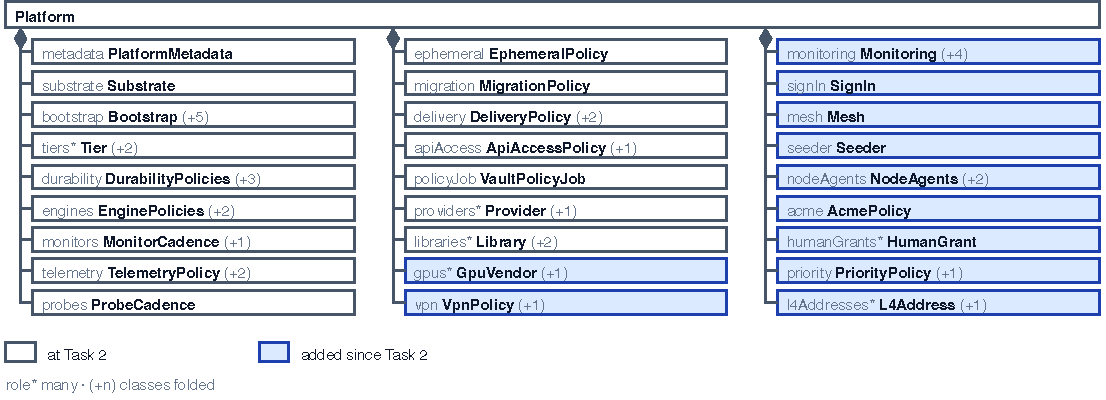
\includegraphics[width=\linewidth, keepaspectratio]{Figures/mm-platform}
\caption{The Platform Intent Metamodel as Submitted}
\label{fig:mm-platform}
\end{figure}

Platform Intent changed in two ways. First, the eight privileged-role fields
now name both a Project and an Application, breaking compatibility with every
document that sets them. Second, it gained policies previously held in
transformations or Project files: the VPN image, GPU resource names, library
grants and each engine's catalog method.

\begin{table}[!htbp]
\centering
\footnotesize
\begin{tabular}{>{\raggedright\arraybackslash}p{\dimexpr0.22\linewidth-2\tabcolsep}>{\raggedright\arraybackslash}p{\dimexpr0.48\linewidth-2\tabcolsep}>{\raggedright\arraybackslash}p{\dimexpr0.30\linewidth-2\tabcolsep}}
\hline
\textbf{Change} & \textbf{What changed} & \textbf{Why} \\
\hline
\multicolumn{3}{l}{\textit{Privileged roles and human access}} \\
Roles name their Project & The eight fields giving an \texttt{Application} a privileged role take \texttt{<project>/<application>}, resolved in \path{ProjectIntentScopes.java}. This breaks compatibility with every Platform Intent. & An Application Id can be declared in any Project's file; a bare Id cannot identify its Project. \\
Human grants & \texttt{humanGrants}: each entry contains a \texttt{group} (as seen by the API server), one of four built-in cluster roles, and a \texttt{reason}. & The platform decides who administers the cluster, so grants belong to no Application. \\
\multicolumn{3}{l}{\textit{Engines}} \\
Catalog method & An engine entry names a \texttt{catalog} method: an image that applies a catalog through the engine's Surface, with its user and sign-in. & Applying a database catalog writes to a live datastore using a privileged identity. The platform specifies each engine's method; the transformation only plans the Job. \\
New engines & \texttt{mongo} joins the engine vocabulary, and \texttt{s3} gains a bucket catalog method. & No catalog is derived for a store without databases; object-store keys and buckets are derived from edges. \\
\multicolumn{3}{l}{\textit{Resources available to Processes}} \\
VPN policy & \texttt{VpnPolicy}: an image, a credential, \texttt{memory} and \texttt{cpu}, and \texttt{VpnSetting} key-value entries. & The tunnel's image and settings are platform facts that no Project should set. \\
GPU vendors & \texttt{GpuVendor} with \texttt{GpuVendorPolicy}: a \texttt{resource} name and a \texttt{runtimeClass}. & The resource name and runtime class belong to the driver the platform runs. \\
Libraries & \texttt{LibraryDeclaration} with \texttt{Library} entries: a directory on one node and the Projects granted access. & The platform names directories and grants access; Projects mount only those granted to them. \\
Substrate pulls & The substrate's image pull is allowed within every derived deadline. & A deadline derived for another purpose must not cause an image pull to fail. \\
\hline
\end{tabular}
\caption{Changes to the Platform Intent Since Task~2: Privileged Roles and Human Access; Engines; Resources Available to Processes}
\label{tab:app-platform}
\end{table}

\begin{table}[!htbp]
\centering
\footnotesize
\begin{tabular}{>{\raggedright\arraybackslash}p{\dimexpr0.22\linewidth-2\tabcolsep}>{\raggedright\arraybackslash}p{\dimexpr0.48\linewidth-2\tabcolsep}>{\raggedright\arraybackslash}p{\dimexpr0.30\linewidth-2\tabcolsep}}
\hline
\textbf{Change} & \textbf{What changed} & \textbf{Why} \\
\hline
Tier forward auth & A tier's \texttt{forwardAuth} names a provider Application, its responding Surface and the path. & The endpoint follows the provider's Process, so moving the provider updates the edge's target. \\
Tier certificates and addresses & A tier gains an L4 Address and its own certificate; a Route takes its TLS from its tier. & Each tier is a proxy with its own entry point and certificate. \\
Tier DNS and ingress class & A tier declares \texttt{dns} (\texttt{target}, \texttt{proxied}) and an ingress class. & Routes carry the annotations required by public records and the selected proxy. \\
Default certificate & A tier that issues no certificate names a Secret Store path in \texttt{certificateFrom}. & Every proxy serves that certificate to a Route naming none of its own. \\
L4 Addresses & Named L4 Addresses, each an IPv4 pool announced at one site. & A raw Surface needs a platform-owned address. \\
Mesh enrolment & \texttt{mesh.enrolled} names the Projects in the ambient mesh. & Enrolment is the platform's decision, and a name no Project declares is rejected. \\
\hline
\end{tabular}
\caption{Changes to the Platform Intent Since Task~2: Tiers, the Edge and the Mesh}
\label{tab:app-platform-2}
\end{table}

\begin{table}[!htbp]
\centering
\footnotesize
\begin{tabular}{>{\raggedright\arraybackslash}p{\dimexpr0.22\linewidth-2\tabcolsep}>{\raggedright\arraybackslash}p{\dimexpr0.48\linewidth-2\tabcolsep}>{\raggedright\arraybackslash}p{\dimexpr0.30\linewidth-2\tabcolsep}}
\hline
\textbf{Change} & \textbf{What changed} & \textbf{Why} \\
\hline
Flux metrics & The bootstrap set's Flux entry records the port and path where its controllers serve metrics. & Flux serves all Projects and belongs to none, so the platform records how to reach it. \\
k3s metrics and monitoring stores & The bootstrap set's \texttt{k3s} entry (\texttt{K3sInstall}, \texttt{K3sMetrics}) records where the kubelet, the API server and the cluster DNS serve metrics; \texttt{Monitoring} gains \texttt{stores}, the Loki, Tempo and Pyroscope Applications Grafana reads. & The cluster's own components and Grafana's data sources belong to no Project, so the platform records them. \\
Priority classes & Two classes, \texttt{data} and \texttt{critical}, and a list of critical Applications. & Priority is derived from the Process rather than authored by it. \\
Node agents & Node agents are derived from node facts and pools. & Agents follow existing nodes without a duplicated list. \\
Foundation and bootstrap set & The remaining foundation and its bootstrap set are declared. & The platform specifies what a cluster needs before any Project runs. \\
Off-cluster recipient & Each off-cluster copy is encrypted to a platform-named recipient. & Only the holder of the recipient's key may read the copy. \\
DNS resolution & A DNS-serving Process resolves through the platform's upstream nameservers. & The resolver's upstream is a platform fact. \\
\hline
\end{tabular}
\caption{Changes to the Platform Intent Since Task~2: Scheduling, Priority and the Foundation}
\label{tab:app-platform-3}
\end{table}

\subsection{Pinned Inputs}
\label{sec:appendix-pinned}

Pinned inputs are documents read during resolution but not written by an author:
the images lock, node contract and ClusterState snapshot. Their classes are
defined in \path{pinned-inputs.ecore} and shown in Figure~\ref{fig:mm-pinned}.
The changes concern the images lock's versions and checks, and the snapshot's
backup list.

\begin{figure}[!htbp]
\centering
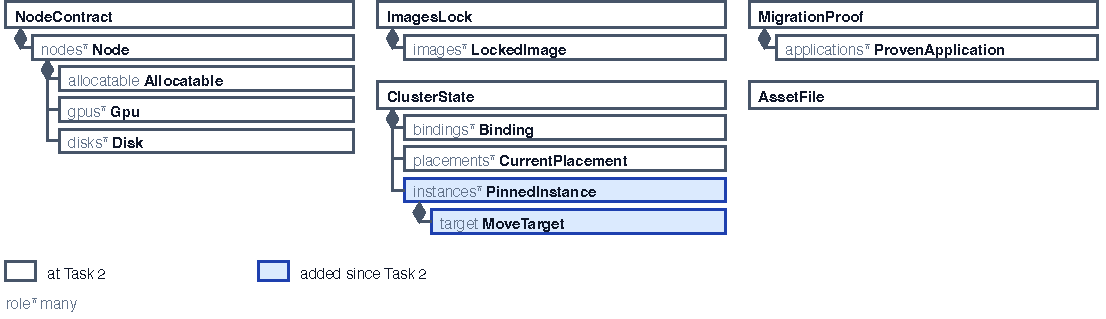
\includegraphics[width=\linewidth, keepaspectratio]{Figures/mm-pinned}
\caption{The Pinned Inputs Metamodel as Submitted}
\label{fig:mm-pinned}
\end{figure}

\begin{table}[!htbp]
\centering
\footnotesize
\begin{tabular}{>{\raggedright\arraybackslash}p{\dimexpr0.22\linewidth-2\tabcolsep}>{\raggedright\arraybackslash}p{\dimexpr0.48\linewidth-2\tabcolsep}>{\raggedright\arraybackslash}p{\dimexpr0.30\linewidth-2\tabcolsep}}
\hline
\textbf{Change} & \textbf{What changed} & \textbf{Why} \\
\hline
\multicolumn{3}{l}{\textit{Images lock}} \\
Version on every entry & Each images-lock entry gains \texttt{version}, a \texttt{String} in \path{pinned-inputs.ecore} and \path{ImagesLock.xtext}. Rendering writes it on every pod running the image. & A pod must identify its software release. \\
Rejection of missing versions & The grammar accepts an entry without \texttt{version}; resolution rejects it as \texttt{E\_IMAGE\_VERSION\_MISSING}. & This identifies the model entry, whereas a grammar error would identify only the line. \\
Root rejected & An image locked with uid 0 is rejected as \texttt{E\_IMAGE\_RUNS\_AS\_ROOT}. & The hardening posture requires a non-root uid, which a root image cannot supply. \\
\multicolumn{3}{l}{\textit{ClusterState snapshot}} \\
Backups removed & The snapshot's rollback-backup list and annotation are removed. & Rollback uses scheduled backups, so the snapshot no longer records an unused backup. \\
\hline
\end{tabular}
\caption{Changes to the Pinned Inputs Since Task~2: Images Lock; ClusterState Snapshot}
\label{tab:app-pinned}
\label{tab:app-pinned-2}
\end{table}

Output remains a function of the pinned inputs. A fact about the running cluster
therefore enters as a new pinned value, rather than a live-cluster read. Section~\ref{sec:design} covers the snapshot rules and the reason the node
contract records capacity; they are not repeated here.

\subsection{Target Metamodel (Resolved Deployment)}
\label{sec:appendix-target}

Resolution produces the Resolved Deployment; rendering reads it. It grew in two
areas: values derived per Project and features required by workloads.
Figure~\ref{fig:mm-target} shows the metamodel. As in Task~2, there is one root
instance per Project, but its values now belong to that Project. In Task~2,
every Project recorded the same Vault policy Job and rollout events. Each now
has its own values, delivered by its own Reconcile Unit.

\begin{figure}[!htbp]
\centering
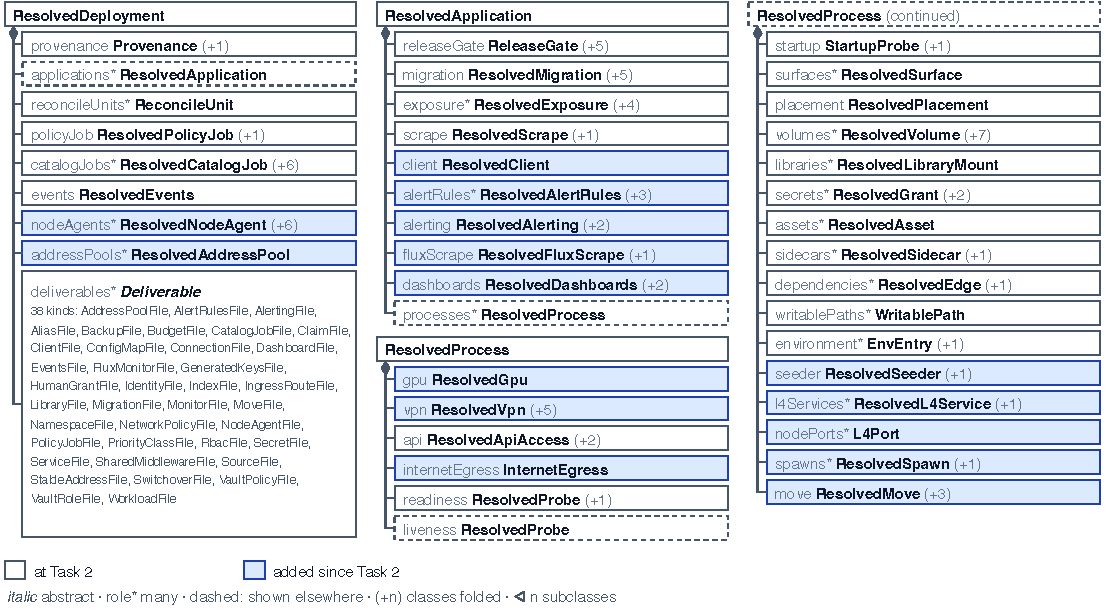
\includegraphics[width=\linewidth, keepaspectratio]{Figures/mm-target}
\caption{The Target Metamodel as Submitted}
\label{fig:mm-target}
\end{figure}

\begin{table}[!htbp]
\centering
\footnotesize
\begin{tabular}{>{\raggedright\arraybackslash}p{\dimexpr0.22\linewidth-2\tabcolsep}>{\raggedright\arraybackslash}p{\dimexpr0.48\linewidth-2\tabcolsep}>{\raggedright\arraybackslash}p{\dimexpr0.30\linewidth-2\tabcolsep}}
\hline
\textbf{Change} & \textbf{What changed} & \textbf{Why} \\
\hline
\multicolumn{3}{l}{\textit{Values planned in the Project's own Reconcile Unit}} \\
Policy Job and rollout events & \texttt{ResolvedDeployment} retains \texttt{policyJob} and rollout events, now containing the Project's own Job, Flux provider and alert. & Each Project's Reconcile Unit writes its policies and reports its rollouts without another Project's values. \\
Catalog Job & \texttt{ResolvedCatalogJob} (\texttt{identity}, \texttt{namespace}, \texttt{image}, \texttt{imageVersion}, \texttt{uid}, \texttt{gid}, \texttt{role}, \texttt{address}, \texttt{memory}, \texttt{cpu}, \texttt{deadline}, \texttt{eligibleNodes}) and \texttt{ResolvedCatalog} (\texttt{host}, \texttt{port}, \texttt{connection}, and \texttt{CatalogDatabase} entries of \texttt{name}, \texttt{owner} and \texttt{data}). & A datastore's catalog Job is planned in the Project running the datastore. Its identity fields mirror the policy Job's. \\
Generated keys & \texttt{GeneratedKeysFile} is rendered as JSON by the policy Job. & The policy Job reads generated values from a file written during rendering. \\
\multicolumn{3}{l}{\textit{Consumer admission and Stable Addresses}} \\
Consumer label & A consuming Process has \texttt{consumes}, the label of each Surface it reaches; the provider's policy admits that label. & Only the new consumer is re-rendered, since the provider's policy already admits the label. \\
Stable Address & A resolved Stable Address holds its \texttt{name}, namespace, \texttt{target} and \texttt{port}. Each alias points to it through an \texttt{externalName}. & Consumers do not know where providers run, so relocating a provider changes one object. \\
\hline
\end{tabular}
\caption{Changes to the Resolved Deployment Metamodel Since Task~2: Values Planned in the Project's Own Reconcile Unit; Consumer Admission and Stable Addresses}
\label{tab:app-target}
\end{table}

\begin{table}[!htbp]
\centering
\footnotesize
\begin{tabular}{>{\raggedright\arraybackslash}p{\dimexpr0.22\linewidth-2\tabcolsep}>{\raggedright\arraybackslash}p{\dimexpr0.48\linewidth-2\tabcolsep}>{\raggedright\arraybackslash}p{\dimexpr0.30\linewidth-2\tabcolsep}}
\hline
\textbf{Change} & \textbf{What changed} & \textbf{Why} \\
\hline
\multicolumn{3}{l}{\textit{Workload features}} \\
Image version on pods & Processes, sidecars and Jobs have \texttt{imageVersion}. & Rendering writes the version on every pod. \\
VPN & \texttt{ResolvedVpn} with \texttt{image}, \texttt{imageVersion}, \texttt{memory}, \texttt{cpu}, \texttt{forwardedPort}, \texttt{environment} and the \texttt{credential}. & The attached Process's tunnel container needs its own image and credential. \\
GPU and libraries & \texttt{ResolvedGpu} (\texttt{resource}, \texttt{runtimeClass}) and \texttt{ResolvedLibraryMount} (\texttt{library}, \texttt{claim}, \texttt{volume}, \texttt{node}, \texttt{path}, \texttt{gid}, \texttt{mountAt}, \texttt{subPath}, \texttt{access}). & The scheduling node and the mounted directory are facts of the pod, not of the Project. \\
Internet egress & \texttt{InternetEgress} records the \texttt{reason} for the exception. & The network policy places each reason beside its rule. \\
Release Gate provider & \texttt{GateProvider} records the Process a gate member waits for and the runner's version. & A gate member starts only after its required Processes in the same Project. \\
\multicolumn{3}{l}{\textit{Process forms and tiers}} \\
Command, memory-backed paths and Flux metrics & \texttt{ResolvedProcess} and \texttt{ResolvedSidecar} gain \texttt{command} and \texttt{arguments}; a writable path gains \texttt{memory}; \texttt{ResolvedApplication} gains \texttt{fluxScrape}. & Each resolves a declaration added to the source. \\
Process forms & \texttt{scheduled} (a CronJob), \texttt{parked}, \texttt{across} anti-affinity, \texttt{spawn} templates and the sidecar's \texttt{init} step. & Each form renders a different workload, and the target records which one it is. \\
Tier entries & The forward-auth endpoint, the Route's redirect Middleware, ingress class and DNS annotations, L4 Service, Client object and human-grant ClusterRoleBinding. & Each entry represents a tier or grant fact in Platform Intent. \\
Priority and node agents & A Process's priority class and the node agents' pools. & Priority is derived; agents are derived from node facts. \\
Monitoring stack and default certificate & \texttt{ResolvedOperated} (with \texttt{OperatedAlertmanager} and \texttt{OperatedFlag}) records a Prometheus or Alertmanager the Prometheus operator runs; \texttt{GrafanaFile} with \texttt{ResolvedGrafana}, \texttt{K3sMonitorsFile} with \texttt{ResolvedK3sScrape}, and \texttt{TlsStoreFile} carry the Grafana instance, the scrapes of k3s and a tier's default certificate; \texttt{ResolvedMemberlist} the node speakers' shared key. & Each object is derived from a platform fact, so the templates only write it. \\
\hline
\end{tabular}
\caption{Changes to the Resolved Deployment Metamodel Since Task~2: Workload Features; Process Forms and Tiers}
\label{tab:app-target-2}
\end{table}

\begin{table}[!htbp]
\centering
\footnotesize
\begin{tabular}{>{\raggedright\arraybackslash}p{\dimexpr0.22\linewidth-2\tabcolsep}>{\raggedright\arraybackslash}p{\dimexpr0.48\linewidth-2\tabcolsep}>{\raggedright\arraybackslash}p{\dimexpr0.30\linewidth-2\tabcolsep}}
\hline
\textbf{Change} & \textbf{What changed} & \textbf{Why} \\
\hline
Capabilities, names and suffix & \texttt{VaultPolicyFile.paths} and \texttt{ResolvedCatalogJob.policy} record each path and its capabilities; \texttt{MiddlewareStep} gains \texttt{name} and \texttt{namespace}; \texttt{ResolvedProcess} gains \texttt{serving} and \texttt{servingLabel} (Table~\ref{tab:moved-choices}). The rendered trees keep their bytes, save one redirect step's name (Section~\ref{sec:m2t-queries}). & A value chosen in a template lies beyond model-level tests. \\
\hline
\end{tabular}
\caption{Changes to the Resolved Deployment Metamodel Specific to the Model-Driven Implementation}
\label{tab:app-target-3}
\end{table}

Every value needed for rendering is recorded in the Resolved Deployment, which
is the only rendering input. Acceleo templates therefore read the consumer label,
version and catalog identity from the model without deriving them.

\subsection{The Transformations}
\label{sec:appendix-transformations}

The pipeline changed from Task~2's lowering, resolution and estate pass over
several Resolved Deployments, followed by rendering, to lower, resolve and
render. The estate pass was removed; resolution now plans its values per
Project. Its ADR, \path{emf/docs/adr/emf/0076-qvto-derives-the-resolved-deployment.md},
was rewritten in place rather than amended, recording the current decision.
It rests on the rule that a Project owns every object it delivers
(\path{docs/adr/model/0116-a-project-owns-every-object-it-delivers.md}).
The record accepts the cost: values needed by several Projects are planned
separately by each.


\begin{table}[!htbp]
\centering
\footnotesize
\begin{tabular}{>{\raggedright\arraybackslash}p{\dimexpr0.22\linewidth-2\tabcolsep}>{\raggedright\arraybackslash}p{\dimexpr0.48\linewidth-2\tabcolsep}>{\raggedright\arraybackslash}p{\dimexpr0.30\linewidth-2\tabcolsep}}
\hline
\textbf{Change} & \textbf{What changed} & \textbf{Why} \\
\hline
\multicolumn{3}{l}{\textit{Pipeline}} \\
estate pass removed & \texttt{estate.qvto}, its runner and tests are removed; the pipeline runs lower, resolve and render. Each Project's resolution plans the values previously planned by the pass. & With each Project owning its objects, no transformation needs to read several Resolved Deployments together. \\
\multicolumn{3}{l}{\textit{Values planned and applied in the Project's own Reconcile Unit}} \\
Vault policy Job & Resolution plans a Job per Project, in its namespace, named by the digest of its own documents. & A Project's Reconcile Unit becomes ready without waiting for a shared Job. \\
Rollout events & Resolution plans a Flux provider and alert per Project, in Flux's namespace, applied by that Project's Reconcile Unit. & Each Project reports its own rollouts. \\
Catalog Job & A datastore's catalog Job, ConfigMap, CronJob and policy are planned into its Project's output, under the Application running it. & The Reconcile Unit that starts the datastore applies its catalog without waiting for another Reconcile Unit. \\
Routes & Each Exposure's Route is written into its Application's directory and applied by its Project's Reconcile Unit, after the Reconcile Unit of the Project declaring the tier's proxy. & A Route depends on its named proxy; the Reconcile Unit graph specifies the order. \\
Job names and recreation & A catalog or policy Job is named by the digest of its inputs and pod template. If only rendering changed the template, the Job is marked for recreation. & Job templates are immutable, so a rendering change retaining the name would stall the Reconcile Unit. \\
Retries and placement & Policy and catalog Jobs retry until an attempt succeeds, with a deadline per attempt, and avoid nodes with SD cards. & A slow disk must not make a slow start permanently fail the Job. \\
\multicolumn{3}{l}{\textit{Consumer admission by label}} \\
Consumer label & Resolution gives each consuming Process the label of each Surface it reaches. The provider's policy admits the label from any namespace; the catalog Job holds its datastore's Surface label. & Adding a consumer re-renders only that consumer, leaving provider policies unchanged. \\
\hline
\end{tabular}
\caption{Changes to the Transformations Since Task~2: Pipeline; Values Planned and Applied in the Project's Own Reconcile Unit; Consumer Admission by Label}
\label{tab:app-transform}
\end{table}

\begin{table}[!htbp]
\centering
\footnotesize
\begin{tabular}{>{\raggedright\arraybackslash}p{\dimexpr0.22\linewidth-2\tabcolsep}>{\raggedright\arraybackslash}p{\dimexpr0.48\linewidth-2\tabcolsep}>{\raggedright\arraybackslash}p{\dimexpr0.30\linewidth-2\tabcolsep}}
\hline
\textbf{Change} & \textbf{What changed} & \textbf{Why} \\
\hline
Generated keys & The Vault policy Job generates each declared key and rejects generated paths escaping its Project's prefix. & The Job owning the path writes the generated value. \\
VPN and library & Each attached Process receives its own VPN credential; library mounts are resolved against the library's node. & Credentials are not shared between Processes, and mounts need their node's path. \\
File backups & A file backup runs as the Process owning the volume. & The backup reads the volume using its owner's identity. \\
Edges and ordering & A \texttt{required: false} edge imposes no Reconcile Unit ordering. A gated member starts only after its required stop-start Processes in the same Project. & Optional edges are not dependencies; a gate must not start before what it gates. \\
Secret Store connection & A datastore's Secret Store connection is named after its Process, not its engine. & Two datastores of one engine must not share a connection. \\
Images & Every locked image's version is read and written on its pods. Every derived deadline allows time for a pull. & Version is a pod fact; no deadline may prevent a pull scheduled by rendering. \\
\hline
\end{tabular}
\caption{Changes to the Transformations Since Task~2: Resolution Rules}
\label{tab:app-transform-2}
\end{table}

\begin{table}[!htbp]
\centering
\footnotesize
\begin{tabular}{>{\raggedright\arraybackslash}p{\dimexpr0.22\linewidth-2\tabcolsep}>{\raggedright\arraybackslash}p{\dimexpr0.48\linewidth-2\tabcolsep}>{\raggedright\arraybackslash}p{\dimexpr0.30\linewidth-2\tabcolsep}}
\hline
\textbf{Change} & \textbf{What changed} & \textbf{Why} \\
\hline
\multicolumn{3}{l}{\textit{Rendering}} \\
Restricted posture & The restricted posture sets \texttt{allowPrivilegeEscalation} to false on every container. & Pod Security's restricted profile requires this; otherwise, a setuid binary could escalate privileges. \\
Grant sync objects & A removed grant's sync objects outlive the release removing it. & A running Process may still read the synced secret during rollout, so these objects must outlive the release. \\
Writable paths & Every sidecar mounts the Process's writable paths. & A sidecar that reads the Process's writes must see them. \\
Rate limit and VPN templates & A Route's rate limit renders as a separate Middleware; a dedicated template renders a Process's VPN container. & Each is a separate object required by the proxy or pod. \\
\multicolumn{3}{l}{\textit{Specific to the model-driven implementation}} \\
Choices derived outside templates & \texttt{middlewareOf} names each step and sets its namespace; \texttt{servesFromPrimary} sets the serving Deployment and its label; \texttt{allowedPaths} and \texttt{ResolvedCatalog::policy} build each policy's paths, also used to write the policy Job's documents. Seven queries leave \texttt{render.mtl}: \texttt{allowsAt}, \texttt{policyPaths}, \texttt{catalogAllows}, \texttt{catalogPaths}, \texttt{middlewareName}, \texttt{rateLimitName} and \texttt{listed}. & Template choices were tested only through bytes. Derived values are model features covered by resolution tests; the policy Job and template read one list rather than deriving it separately. \\
Kind dispatch and failure & YAML kinds dispatch by type rather than a chain of type tests. Rendering writes files to a separate directory and moves them under the root only after all files are written. & A kind without a template fails the run; failure leaves the root unchanged. \\
\hline
\end{tabular}
\caption{Changes to the Transformations Since Task~2: Rendering; Changes Specific to the Model-Driven Implementation}
\label{tab:app-transform-3}
\end{table}

\begin{table}[!htbp]
\centering
\footnotesize
\begin{tabular}{>{\raggedright\arraybackslash}p{\dimexpr0.22\linewidth-2\tabcolsep}>{\raggedright\arraybackslash}p{\dimexpr0.48\linewidth-2\tabcolsep}>{\raggedright\arraybackslash}p{\dimexpr0.30\linewidth-2\tabcolsep}}
\hline
\textbf{Change} & \textbf{What changed} & \textbf{Why} \\
\hline
\multicolumn{3}{l}{\textit{Stable Addresses}} \\
Stable Address & Each Surface named by an edge or a tier's forward auth receives a derived Stable Address, rendered as one \texttt{ExternalName} Service. Aliases point to it. & Relocating a provider changes one object, without changing consumer configuration. \\
\multicolumn{3}{l}{\textit{Process forms and the Release Gate}} \\
Process forms & Scheduled Processes render a CronJob forbidding overlap; parked Processes retain claims; replicas spread across nodes; spawn templates bound the pods a Process creates. & The Process declaration fixes each form's behaviour, rather than a rendering flag. \\
Release Gate decisions & The Release Gate decides whether to roll back a release it can no longer pass. & The observing gate decides whether a release can still pass. \\
\hline
\end{tabular}
\caption{Changes to the Transformations Since Task~2: Stable Addresses; Process Forms and the Release Gate}
\label{tab:app-transform-4}
\end{table}

\begin{table}[!htbp]
\centering
\footnotesize
\begin{tabular}{>{\raggedright\arraybackslash}p{\dimexpr0.22\linewidth-2\tabcolsep}>{\raggedright\arraybackslash}p{\dimexpr0.48\linewidth-2\tabcolsep}>{\raggedright\arraybackslash}p{\dimexpr0.30\linewidth-2\tabcolsep}}
\hline
\textbf{Change} & \textbf{What changed} & \textbf{Why} \\
\hline
Flux metrics and metrics egress & The metrics stack's Project renders one PodMonitor for Flux in its own namespace; egress is derived to every declared scrape port and Flux's port. A memory-backed path adds its size to the Process's request, limit and eligibility. & The monitor and egress follow declared facts without manual specification. \\
Human grants & Each grant renders one ClusterRoleBinding from its role to its group, named for both. & Grants belong to no Project, so rendering or removing a Project cannot remove them. \\
Tiers & The tier entry determines its proxy configuration, forward-auth Middleware, shared Middlewares, Route TLS and DNS annotations. & A Route reaches exactly one proxy, selected by its audience. \\
Monitoring stack & Resolution derives the operator's objects for Prometheus and Alertmanager, the Grafana instance, the scrapes of k3s with their token and read access, and each tier's default TLS store. & Each follows a Platform Intent fact rather than a Project's declaration. \\
Encryption and resolver & Off-cluster copies are encrypted to the platform's recipient; DNS-serving Processes use the upstream nameservers. & Rendering uses both platform facts as given. \\
\hline
\end{tabular}
\caption{Changes to the Transformations Since Task~2: Platform Policies and Tiers}
\label{tab:app-transform-5}
\end{table}

Each change was made in the specification and in both implementations, without
generating either implementation from the other. Committed oracle files hold
both to the same result (Section~\ref{sec:evaluation}); this appendix only
records the changes.

\section{The Production Implementation}
\label{sec:appendix-production}

The production implementation, in TypeScript under \path{src/}, compiles the same
model for production use. It renders the same cases, and
\path{test/model/render.test.ts} compares its output with the same committed files.
Its serialiser writes YAML with \texttt{version: "1.1"}
(\path{src/infrastructure/serializer.ts}), the rule the templates' quoting follows
(Section~\ref{sec:design}). The repository forbids generating either implementation
from the other, and regenerating an oracle in CI. Where the two disagreed, the
difference was a defect in one of them: each time the production implementation
gained a rule, the model-driven implementation adopted it until both matched the
oracles.

This independence is partial: one author wrote both implementations, and the
committed trees changed in the same commits as an implementation. A self-generated
snapshot accepts defects present when it was taken; a shared expected tree exposes
disagreements between implementations. Agreement rules out errors made by only one
implementation, but cannot rule out a shared misreading of the specification.
External checks address part of this remaining risk: schemas, profiles and clusters
check Kubernetes requirements rather than the project's specification. Each check has
limits: byte equality establishes expected text rather than correctness; schemas
cannot establish that a \texttt{NetworkPolicy} permits the intended traffic; dry-runs
reveal nothing about controller behaviour. The Pod Security check permits one named
exception: the VPN sidecar.
% TODO(verify): confirm the review of committed trees was by the author alone

% BIB: none needed in this section.
